\documentclass[12pt]{article}

\usepackage[a4paper,margin=1in]{geometry}
\usepackage{amsmath,amssymb}
\usepackage{array}
\usepackage{booktabs}
\usepackage{enumitem}
\usepackage{graphicx}
\usepackage{hyperref}
\usepackage{xcolor}

\hypersetup{
  colorlinks=true,
  linkcolor=black,
  citecolor=blue!50!black,
  urlcolor=blue!50!black
}

\newcolumntype{L}[1]{>{\raggedright\arraybackslash}p{#1}}
\setlength{\emergencystretch}{2em}
\setcounter{tocdepth}{2}

\title{\textbf{A Readout-Covariance Classifier for Shared-Parent Tau Core Signals}\\
\large Synthetic Methodology, Two-Axis Evidence Hierarchy, and Lensing--Morphology Protocol}
\author{Tau Core Research}
\date{Paper 17 draft package, 2026}

\begin{document}
\maketitle

\begin{abstract}
Tau Core is a readout-based research program in which observed physical
descriptions are treated as sector readouts of a deeper parent morphological
body.  A central methodological risk is that apparent morphology or orientation
agreement between two residual channels can be mistaken for evidence of a
shared parent source.  This paper packages a synthetic readout-covariance
classifier that separates these two axes.

The diagnostic plane is
\[
  (Z_{\rm shared},Z_{\rm orient}),
\]
where \(Z_{\rm shared}\) measures shared-parent cross-readout covariance and
\(Z_{\rm orient}\) measures morphology/orientation-like structure.  The claim
boundary is strict: shared-parent covariance is the primary synthetic evidence
axis, while morphology/orientation is only conditional reinforcement.  A signal
with \(Z_{\rm orient}>2\) but \(Z_{\rm shared}\leq3\) is classified as
orientation-only and is not Tau Core evidence.

The included v11 audit contains \(270\) synthetic runs, split evenly into
\(135\) TauWorld and \(135\) NullWorld cases across ten seed values.  All
TauWorld runs recover the shared-parent axis, while the independent-parent
NullWorld has zero shared-parent false positives in this sample.  The same
NullWorld nevertheless exhibits orientation-only structure in \(31/135\) cases,
or \(22.963\%\).  The main methodological result is therefore not that TauWorld
succeeds, since TauWorld is generated with a shared parent.  The result is that
orientation can be visually or morphologically suggestive in null worlds
without becoming shared-parent evidence.  The package therefore supports a
two-axis reporting standard for future lensing, galaxy, cosmic-web, and
weak-signal Tau Core tests.

These numbers are synthetic audit statistics.  They are not \(p\)-values,
likelihood ratios, real-data detections, or physical validation of Tau Core.
The paper's contribution is a reproducible classifier and evidence hierarchy
that complements Paper 14's cosmic-web witness ladder and Paper 16's
weak-signal amplification protocol.
\end{abstract}

\tableofcontents

\section{Scope and claim boundary}

This manuscript should be evaluated as a synthetic methodology and
claim-boundary paper.  It does not analyze real survey products, does not
validate a lensing or cosmic-web anomaly, and does not prove Tau Core.

\noindent\textbf{Status:} synthetic methodology, classifier package, and
protocol formalization.

The main claim is deliberately narrow:
\begin{quote}
In a controlled synthetic package, a two-axis diagnostic can separate
shared-parent readout covariance from orientation-only morphology-like
structure.  Shared-parent covariance is the primary evidence axis;
orientation is secondary and conditional.
\end{quote}

The paper does not claim that dark matter is solved, dark energy is explained,
galaxy rotation residuals are explained, lensing residuals are detected, or a
physical Tau parent has been identified.  It only states that the included
synthetic lineage gives a useful audit grammar for future multi-readout tests.

\section{Why this paper is separate from Papers 14 and 16}

Paper 14 defines a cosmic-web witness ladder: galaxy-only filamentarity is not
enough, while galaxy/lensing web-tensor alignment plus redshift stability,
systematics survival, mock rarity, and optionally a third readout gives a
stronger source-frozen candidate route.  Paper 16 defines WSAP, the Weak-Signal
Amplification Protocol: several weak heterogeneous readouts may jointly recover
a hidden parent component better than any single readout.

Paper 17 sits between them.  It asks a more specific question:
\begin{quote}
How do we distinguish shared-parent covariance from morphology/orientation
agreement that can also occur in null worlds?
\end{quote}

The answer is the two-axis classifier:
\[
  (Z_{\rm shared},Z_{\rm orient}).
\]
This classifier is not a replacement for Paper 14 or Paper 16.  It supplies a
missing diagnostic layer.  Paper 14 needs it because cosmic-web morphology can
look convincing even when the shared-parent axis is absent.  Paper 16 needs it
because weak-signal recovery must distinguish shared-parent coherence from
kernel-specific visual alignment.

\section{Parent-readout covariance formalism}

The synthetic package uses a parent-readout skeleton.  Let
\[
  \mathfrak{P}_{\tau}
  =
  (\mathcal{P}_{\tau},\eta_{\tau},H_{\tau},
  \mathcal{A}_{\tau},\Sigma_{\tau})
\]
denote a parent state package, where \(\mathcal{P}_{\tau}\) is the parent state
space, \(\eta_{\tau}\) is a parent pairing, \(H_{\tau}\) is a parent generator,
\(\mathcal{A}_{\tau}\) is a parent observable algebra, and
\(\Sigma_{\tau}\) is a parent perturbation covariance.

The package intentionally allows parent-level indefiniteness.  A toy parent
pairing can be
\[
  \eta_{\tau}=
  \begin{pmatrix}
  1&0\\
  0&-1
  \end{pmatrix}.
\]
For a parent vector
\[
  \Psi_{\tau}=
  \begin{pmatrix}
  \psi_{+}\\
  \psi_{-}
  \end{pmatrix},
\]
the parent norm is
\[
  \langle \Psi_{\tau},\Psi_{\tau}\rangle_{\eta}
  =
  |\psi_{+}|^2-|\psi_{-}|^2.
\]
This quantity may be positive, null, or negative at the parent level.  The
claim-safe rule is not that every parent direction is physical.  The rule is
that physical readouts must be positive after projection.

\subsection{Readout positivity}

A readout channel is represented by a projector
\[
  \Pi_i:\mathcal{P}_{\tau}\to\mathcal{P}_{\tau}.
\]
The induced readout pairing is
\[
  \eta_i=\Pi_i^{\dagger}\eta_{\tau}\Pi_i.
\]
The admissibility condition is
\[
  \boxed{\Pi_i^{\dagger}\eta_{\tau}\Pi_i\geq0.}
  \label{eq:readout-positivity}
\]
This is the readout-positivity principle used in the package.  It is a
synthetic admissibility rule, not a proof that the physical universe has an
indefinite parent metric.

\subsection{Residual channels}

For channel \(i\), a residual is modeled as
\[
  \delta_i(t)
  =
  M_i\Pi_iU_{\tau}(t)\delta\Psi_{\tau}(0)+n_i(t),
  \label{eq:channel-residual}
\]
where \(M_i\) is a response or measurement operator, \(U_{\tau}(t)\) is parent
transport, \(\delta\Psi_{\tau}(0)\) is a parent perturbation, and \(n_i(t)\)
collects channel noise and systematics.

The predicted cross-readout covariance is
\[
  \boxed{
  {\rm Cov}_{ij}(t,t')
  =
  M_i\Pi_iU_{\tau}(t)
  \Sigma_{\tau}
  U_{\tau}^{\dagger}(t')
  \Pi_j^{\dagger}M_j^{\dagger}
  +
  N_{ij}(t,t').
  }
  \label{eq:cross-readout-covariance}
\]
This is the central empirical target of the package.  A Tau Core candidate is
not a single nonzero residual; it is structured covariance between readout
residuals after null, noise, source-overlap, and systematics controls.

\section{Evidence hierarchy}

The paper uses the following hierarchy.

\begin{enumerate}[leftmargin=1.4em]
\item A single residual anomaly is insufficient.
\item Morphology/orientation agreement is insufficient.
\item Shared-parent covariance is candidate synthetic evidence.
\item Shared-parent covariance plus morphology/orientation is stronger
candidate support.
\item Out-of-sample multi-survey survival is required for empirical seriousness.
\item Physical closure requires independently constrained parent states,
projectors, response operators, dynamics, and units.
\end{enumerate}

The warning is simple:
\[
  Z_{\rm orient}>2
  \quad\not\Rightarrow\quad
  \hbox{Tau Core candidate}.
\]
The primary condition is instead
\[
  Z_{\rm shared}>3.
\]

\section{Synthetic lensing--morphology setup}

The first demonstrator uses two residual handles:
\[
  \delta_L \times \delta_F,
\]
where \(\delta_L\) is a lensing-like residual and \(\delta_F\) is a
filament/morphology-like residual.

The toy parent kernel is anisotropic:
\[
  K_{\tau}(r_{\parallel},r_{\perp})
  =
  A_{\tau}^2
  \exp\left[
  -\frac{r_{\parallel}^2}{2\ell_{\parallel}^2}
  -\frac{r_{\perp}^2}{2\ell_{\perp}^2}
  \right],
  \label{eq:parent-kernel}
\]
with filamentary condition
\[
  \ell_{\parallel}>\ell_{\perp}.
\]

Two synthetic worlds are compared:
\[
  P_{\tau}\to\delta_L,\qquad P_{\tau}\to\delta_F
\]
for TauWorld, and
\[
  P_L\to\delta_L,\qquad P_F\to\delta_F,\qquad P_L\perp P_F
\]
for NullWorld.

The test is not whether the two residual maps look similar.  The test is
whether they show source-shared covariance beyond surrogate controls.

\section{From v8 to v11}

The package records a four-step synthetic lineage.

\subsection{v8: shared-parent strength detector}

The v8 strength score was
\[
  S_{\rm shared}
  =
  \sum_{\Delta}|C_{\parallel}(\Delta)|
  +
  \sum_{\Delta}|C_{\perp}(\Delta)|.
\]
The surrogate-normalized score was
\[
  Z_{\rm shared}
  =
  \frac{S_{\rm true}-\mu(S_{\rm sur})}
  {\sigma(S_{\rm sur})}.
\]
This recovered the shared-parent axis strongly in TauWorld and remained near
zero in NullWorld, but the combined v8 rule mixed strength and anisotropy too
aggressively.

\subsection{v9: matched-filter anisotropy rejection}

The v9 attempt tried to make anisotropy more specific.  The result was
rejected as a primary detector: anisotropy can be unstable and can underperform
as a standalone evidence axis.

\subsection{v10: orientation diagnostic}

The v10 step retained orientation as a diagnostic rather than a primary
detector.  It measured orientation-like support while no longer allowing that
axis to substitute for shared-parent covariance.

\subsection{v11: two-axis classifier}

The v11 classifier merges the v8 shared-parent axis and v10 orientation axis.
It reports four classes:
\[
\begin{array}{ll}
A: & Z_{\rm shared}>3,\quad Z_{\rm orient}>2,\\
B: & Z_{\rm shared}>3,\quad Z_{\rm orient}\leq2,\\
C: & Z_{\rm shared}\leq3,\quad Z_{\rm orient}>2,\\
D: & Z_{\rm shared}\leq3,\quad Z_{\rm orient}\leq2.
\end{array}
\]
Classes A and B are shared-parent candidate classes in the synthetic grammar.
Class C is orientation-only and is explicitly not Tau Core evidence.  Class D
is null.

\begin{figure}[t]
\centering
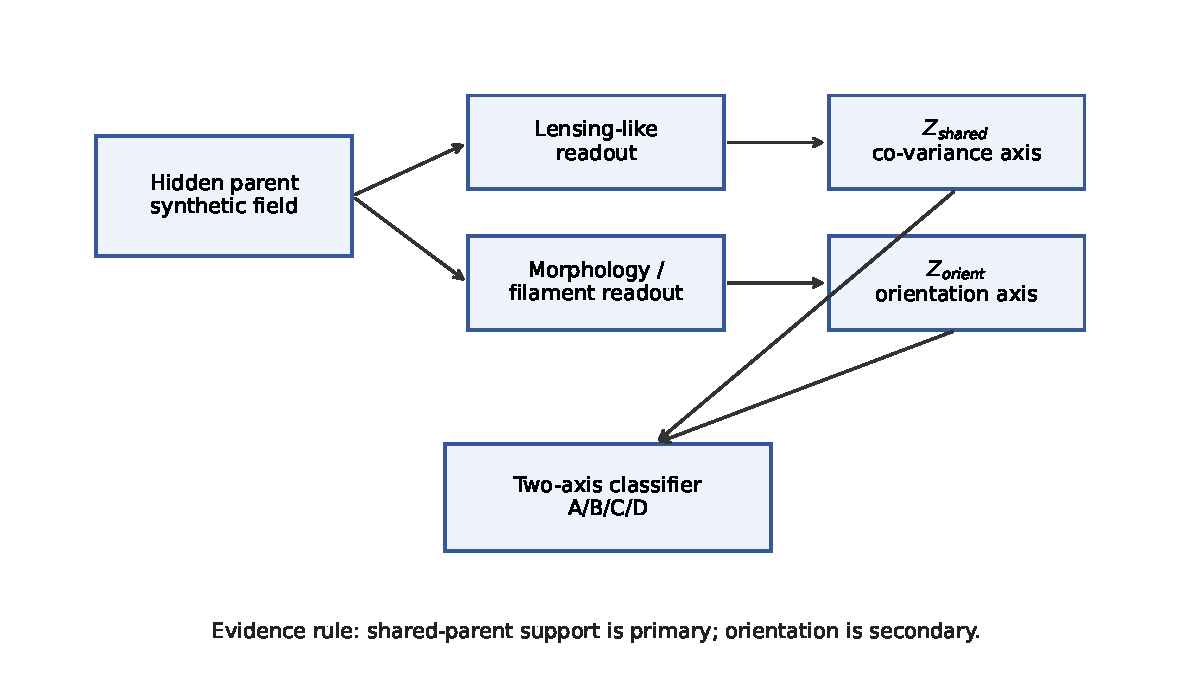
\includegraphics[width=0.95\linewidth]{figures/fig_readout_covariance_protocol.pdf}
\caption{Paper 17 diagnostic structure.  A hidden synthetic parent produces
two residual readouts.  The classifier separates the shared-parent covariance
axis from the morphology/orientation axis before assigning A/B/C/D classes.}
\label{fig:protocol}
\end{figure}

\section{Numerical summary}

The headline v11 summary is shown in Table~\ref{tab:v11-summary}.  The key
point is not that TauWorld succeeds; TauWorld was generated with a shared
parent.  The point is that NullWorld has zero shared-parent false positives
while still producing orientation-only cases.

The compact v11 audit contains \(270\) synthetic runs: \(135\) TauWorld and
\(135\) NullWorld cases, generated from ten distinct seed values
\((11,\ldots,10055)\).  Using Wilson \(95\%\) binomial intervals, the
TauWorld shared-parent recovery rate is \(135/135\), with interval
\([0.972,1.000]\).  The NullWorld shared-parent false-positive rate is
\(0/135\), with interval \([0.000,0.028]\).  The NullWorld orientation-only
rate is \(31/135\), with interval \([0.167,0.307]\).  These intervals are
audit uncertainty summaries for the synthetic package, not empirical
confidence intervals for nature.

\begin{table}[t]
\centering
\small
\begin{tabular}{L{0.42\linewidth}L{0.22\linewidth}L{0.22\linewidth}}
\toprule
Quantity & TauWorld & NullWorld\\
\midrule
Shared-parent recovery rate & 1.000 & 0.000\\
Orientation detection rate & 0.489 & 0.230\\
Mean \(Z_{\rm shared}\) & 6.553 & 0.267\\
Mean \(Z_{\rm orient}\) & 2.401 & 1.020\\
Median \(Z_{\rm shared}\) & 6.275 & 0.202\\
Median \(Z_{\rm orient}\) & 1.939 & 0.320\\
\bottomrule
\end{tabular}
\caption{v11 two-axis classifier summary from the compact synthetic audit
tables.  Values are synthetic audit statistics, not empirical detection
statistics.}
\label{tab:v11-summary}
\end{table}

The class rates are:
\[
\begin{array}{lcc}
\hbox{class} & \hbox{TauWorld} & \hbox{NullWorld}\\
\hline
A\ \hbox{shared+orientation} & 0.489 & 0.000\\
B\ \hbox{shared only} & 0.511 & 0.000\\
C\ \hbox{orientation only} & 0.000 & 0.230\\
D\ \hbox{null} & 0.000 & 0.770.
\end{array}
\]

\begin{figure}[t]
\centering
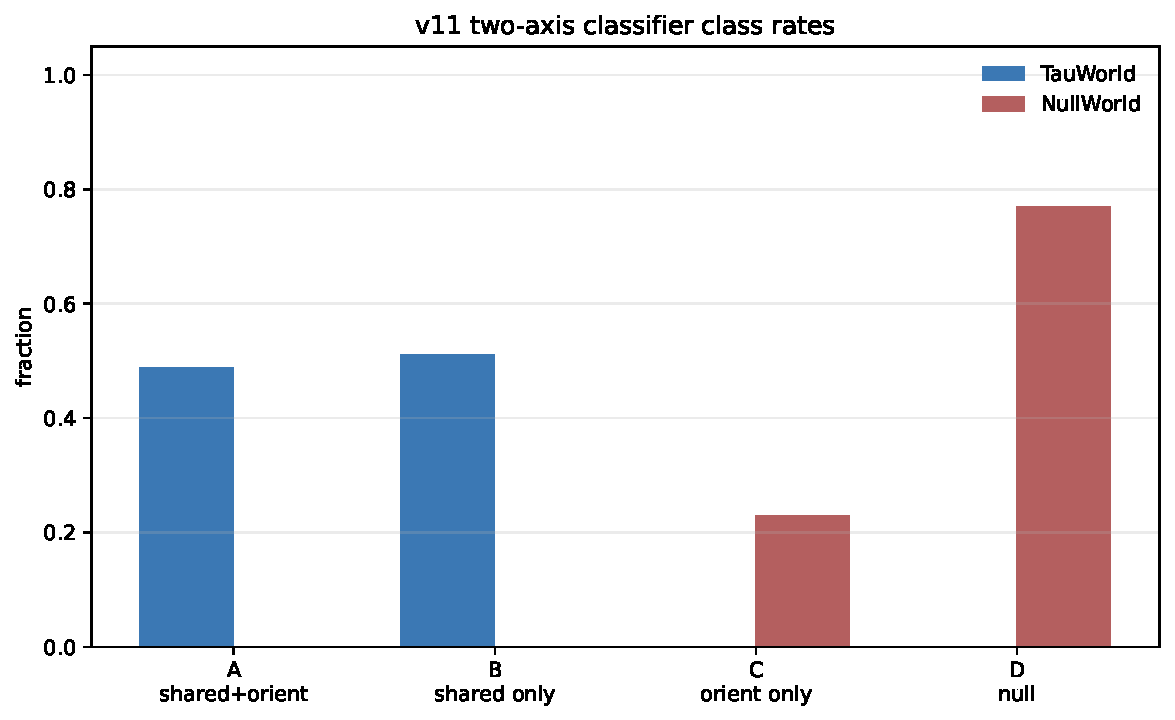
\includegraphics[width=0.88\linewidth]{figures/fig_v11_class_rates.pdf}
\caption{v11 classifier class rates.  TauWorld cases all land in shared-parent
classes A or B.  NullWorld cases never land in A or B, but can land in the
orientation-only class C.}
\label{fig:class-rates}
\end{figure}

\begin{figure}[t]
\centering
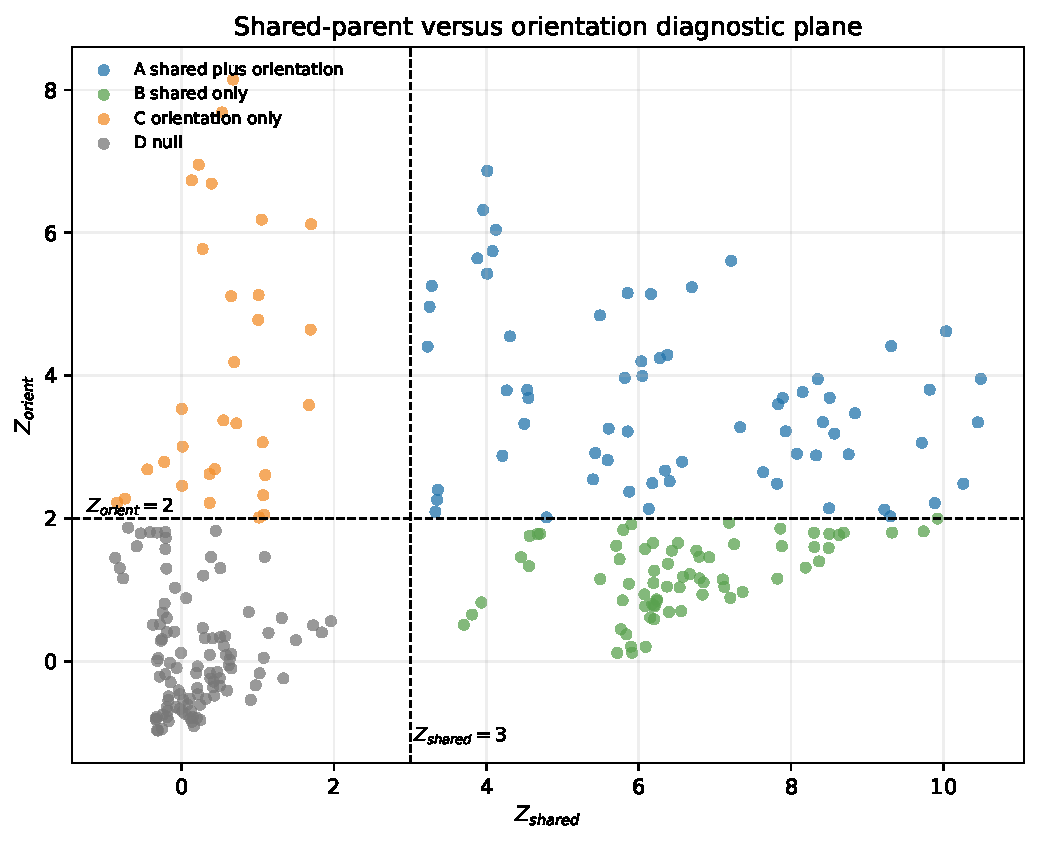
\includegraphics[width=0.88\linewidth]{figures/fig_v11_shared_orient_scatter.pdf}
\caption{The two-axis diagnostic plane.  The vertical line marks
\(Z_{\rm shared}=3\); the horizontal line marks \(Z_{\rm orient}=2\).  The
upper-left region is the warning class: orientation-like structure without
shared-parent support.}
\label{fig:scatter}
\end{figure}

\begin{figure}[t]
\centering
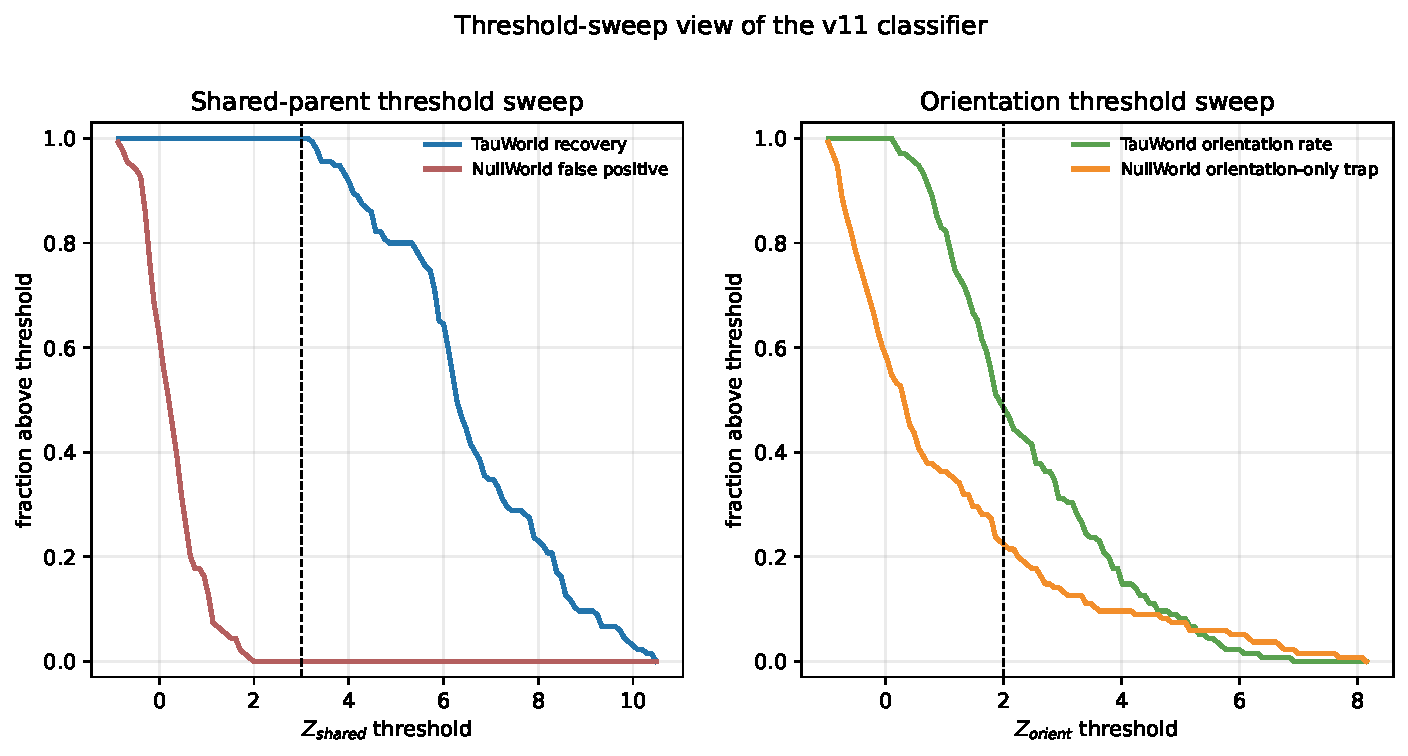
\includegraphics[width=0.95\linewidth]{figures/fig_v11_threshold_sweep.pdf}
\caption{Threshold-sweep view of the v11 classifier.  The left panel varies
the shared-parent threshold and reports TauWorld recovery versus NullWorld
false positives.  The right panel varies the orientation threshold and shows
why orientation is a useful but unsafe secondary axis: NullWorld can produce
orientation-only support over a range of thresholds.  This figure is a
threshold-sensitivity diagnostic, not a validation ROC curve on real data.}
\label{fig:threshold-sweep}
\end{figure}

\section{Why orientation is secondary}

The synthetic audit shows that morphology/orientation structure is useful but
dangerous.  It is useful because a genuine shared parent can have an anisotropic
or filamentary shape, so orientation can reinforce the diagnosis.  It is
dangerous because orientation-like statistics may also arise in independent
parent worlds.

This is why the paper refuses the shortcut
\[
  \hbox{orientation-like morphology}
  \Rightarrow
  \hbox{Tau Core signal}.
\]
The accepted synthetic implication is weaker:
\[
  Z_{\rm shared}>3
  \Rightarrow
  \hbox{shared-parent candidate support},
\]
and
\[
  Z_{\rm shared}>3,\quad Z_{\rm orient}>2
  \Rightarrow
  \hbox{stronger synthetic candidate support}.
\]

Figure~\ref{fig:heatmap} shows how the class-A rate varies across synthetic
conditions.  The condition dependence is a feature, not a bug: the orientation
axis is morphology-dependent and should not be treated as a universal scalar
detector.

\begin{figure}[t]
\centering
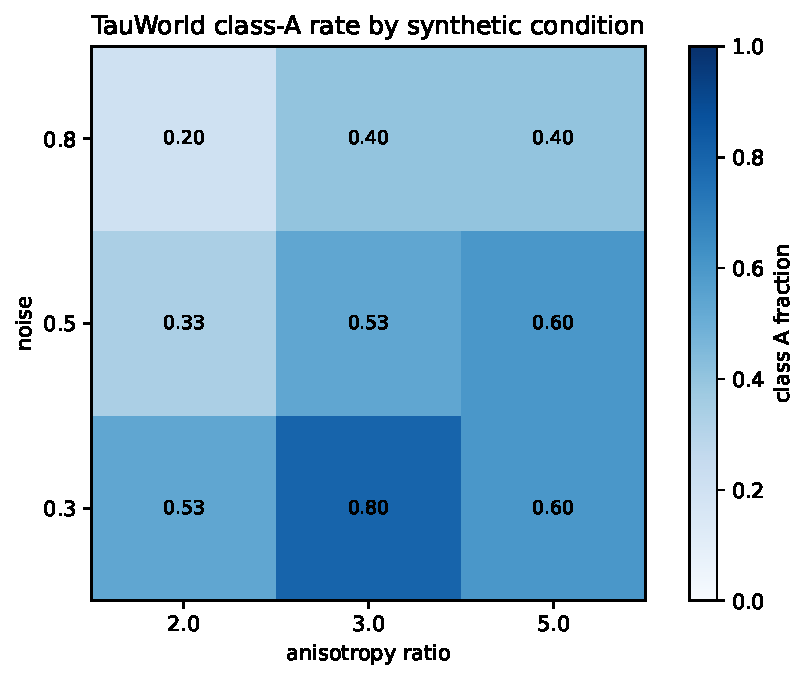
\includegraphics[width=0.78\linewidth]{figures/fig_tauworld_condition_heatmap.pdf}
\caption{TauWorld class-A rate by synthetic anisotropy ratio and noise level.
Orientation reinforcement is condition-dependent; the shared-parent axis is the
primary support axis.}
\label{fig:heatmap}
\end{figure}

\section{Claim-safe real-data protocol}

A real-data version would need source-native residuals:
\[
  \delta_L=L_{\rm obs}-L_{\rm base},
  \qquad
  \delta_F=F_{\rm obs}-F_{\rm base}.
\]
The baselines must include ordinary modeling, survey masks, shape noise,
photo-\(z\) uncertainty, intrinsic alignments, baryonic corrections, and matched
mock or null catalogues where relevant \cite{KiDS1000,ACTDR6Lensing,DESI2016}.

The target statistic would be a residual cross-correlation
\[
  C_{LF}(r_{\parallel},r_{\perp},z)
  =
  \langle
  \delta_L(x,z)\delta_F(x+r,z)
  \rangle,
\]
converted into the two diagnostic axes
\[
  (Z_{\rm shared},Z_{\rm orient})
\]
under predeclared surrogates.

Required null tests include:
\begin{enumerate}[leftmargin=1.4em]
\item phase randomization;
\item map rotation;
\item orientation randomization;
\item redshift-block shuffle;
\item mask-only surrogate;
\item family permutation;
\item independent-parent synthetic null;
\item train/test split.
\end{enumerate}

Only classes A and B can be treated as Tau Core candidate classes.  Class C is
a warning class.  It says that the morphology/orientation axis was activated
without shared-parent covariance.

\section{Relation to WSAP}

Paper 16 showed a broader weak-signal amplification lesson: several weak,
heterogeneous synthetic readouts can jointly recover a shared parent better
than any single readout under controls.  Paper 17 is more specific.  It says
that the joint recovery must be decomposed into at least two axes:
\[
  Z_{\rm shared}
  \quad\hbox{and}\quad
  Z_{\rm orient}.
\]

This prevents an important failure mode.  A visually convincing morphology
match can be a class-C result.  In a WSAP language, that means the apparent
readout agreement is not yet a shared-parent recovery.  Future WSAP packages
should therefore report orientation-like or morphology-like support as a
conditional diagnostic, not as a substitute for shared-parent recovery.

\section{Relation to the Tau-web protocol}

Paper 14's cosmic-web witness ladder has the structure
\[
  W_{\rm clean,gal}
  \parallel
  W_{\rm clean,lens}
  +
  z\hbox{-stability}
  +
  \hbox{systematics survival}
  +
  \hbox{mock rarity}.
\]
Paper 17 clarifies how this should be scored.  A galaxy/lensing alignment can
activate the orientation axis, the shared-parent axis, or both.  If it activates
only \(Z_{\rm orient}\), it remains below Tau-compatible candidate status.

The same rule applies to later photon-lensing MAR templates.  A statistic such
as \(T_{\tau}=B_{\rm env}A_fM_{bf}\), even when extended to convergence/shear
mock channels or a toy lensing/matter residual link, can be a useful
source-frozen lensing/morphology search handle, but its raw correlation with a
lensing residual is not enough.  Without shared-parent covariance survival it
is a \(Z_{\rm orient}\)-type signal, not a \(Z_{\rm shared}\)-type signal.

Thus the Paper 14 witness ladder should treat the Paper 17 classifier as an
internal guard:
\[
  \hbox{web alignment}
  \to
  (Z_{\rm shared},Z_{\rm orient})
  \to
  \hbox{A/B/C/D status}.
\]

\section{Limitations}

The package has important limitations.

\begin{enumerate}[leftmargin=1.4em]
\item The data are synthetic.
\item The parent fields are generated by the package rather than inferred from
external source data.
\item The projectors are modeled, not derived from Tau base principles.
\item The response operators are not physical survey operators.
\item The covariance model is a toy covariance model.
\item The thresholds \(Z_{\rm shared}=3\) and \(Z_{\rm orient}=2\) are synthetic
audit thresholds, not universal constants.
\item The present package reports a threshold-sweep diagnostic, but not a full
ROC/PR validation suite with independent realistic mocks.
\item No real survey covariance, no blind holdout survey, and no physical
amplitude calibration are included.
\end{enumerate}

These limitations do not invalidate the methodological result.  They define its
scope.

\section{Required v13 upgrade}

The next meaningful upgrade is not a stronger claim.  It is a harder mock test.
For Paper17-style evidence to move beyond the current toy world, a v13 package
should be treated as a minimum scientific gate, not an optional polish step.  It
should use:
\begin{enumerate}[leftmargin=1.4em]
\item clustered density fields;
\item filament skeleton extraction;
\item lensing-like projection;
\item survey mask;
\item photo-\(z\) noise;
\item shape noise;
\item galaxy bias;
\item train/test split;
\item independently generated null and shared-parent mock catalogues.
\item threshold-free ROC/PR-style curves and explicit seed/split sensitivity;
\item confidence intervals and failure-rate reporting for all headline rates;
\item harder NullWorlds with common survey mask, common selection bias,
foreground or systematics templates, common smoothing kernels, and partial
parent-leakage controls;
\item an independent implementation of the same frozen classifier.
\end{enumerate}

The v11 classifier should then be applied unchanged.  If the classifier only
works in the current toy generator and fails in realistic mocks, that failure
must be preserved.  If it survives, the branch becomes ready for a
source-frozen real-data endpoint design, not for immediate physical validation.

\section{Reproducibility package}

The repository provides:
\[
  \texttt{python scripts/reproduce.py}.
\]
This command rebuilds the summary artifacts, regenerates paper figures,
compiles the PDF, builds the arXiv source zip, and runs public package tests.

The compact source tables are under
\[
  \texttt{data/derived/}.
\]
The original package manifest and README are preserved under
\[
  \texttt{source\_package\_manifest/}.
\]
The reproduction package intentionally excludes broad private workbench logs and
does not include real survey products.

\section{Conclusion}

Paper 17 records a synthetic readout-covariance classifier for Tau Core
multi-readout tests.  Its main result is not a physical discovery.  Its main
result is a disciplined evidence hierarchy:
\[
  \boxed{
  \hbox{shared-parent covariance first; orientation second.}
  }
\]
The v11 synthetic audit recovers the shared-parent axis in all TauWorld cases
and produces zero shared-parent false positives in NullWorld, while still
showing that orientation-only NullWorld cases exist.  This is exactly the
failure mode the classifier is designed to expose.

The paper therefore strengthens the Tau Core architecture at the methodology
level.  It makes future lensing, galaxy, cosmic-web, and WSAP-style tests less
likely to overread morphology-like agreement.  It does not validate Tau Core,
does not identify the parent field, and does not close the physical response
operator problem.  The next scientific step is a realistic mock-catalog
injection test with the same two-axis classifier frozen in advance.

\bibliographystyle{plain}
\bibliography{refs}

\end{document}
